% One-page architecture figure drawn in TikZ. Boxes name repository code; settings as read 14 Nov 2026.
\documentclass[10pt,a4paper]{article}
\usepackage[margin=9mm]{geometry}
\usepackage{tikz}
\usetikzlibrary{arrows.meta,positioning,calc,fit,backgrounds}
\pagestyle{empty}
\definecolor{ink}{HTML}{17324D}
\definecolor{custom}{HTML}{E6F0FA}
\definecolor{provided}{HTML}{EEEEEE}
\definecolor{guard}{HTML}{E5F2E6}
\definecolor{modelc}{HTML}{FCEBD3}
\definecolor{human}{HTML}{F3E8FA}
\begin{document}
\centering
{\Large\bfseries kcwarni: rules first, models last, every change a test}\par
\small Week 08 / 24522014 \quad Settings as read 14 November 2026; limits change during the round\par
\vspace{2mm}
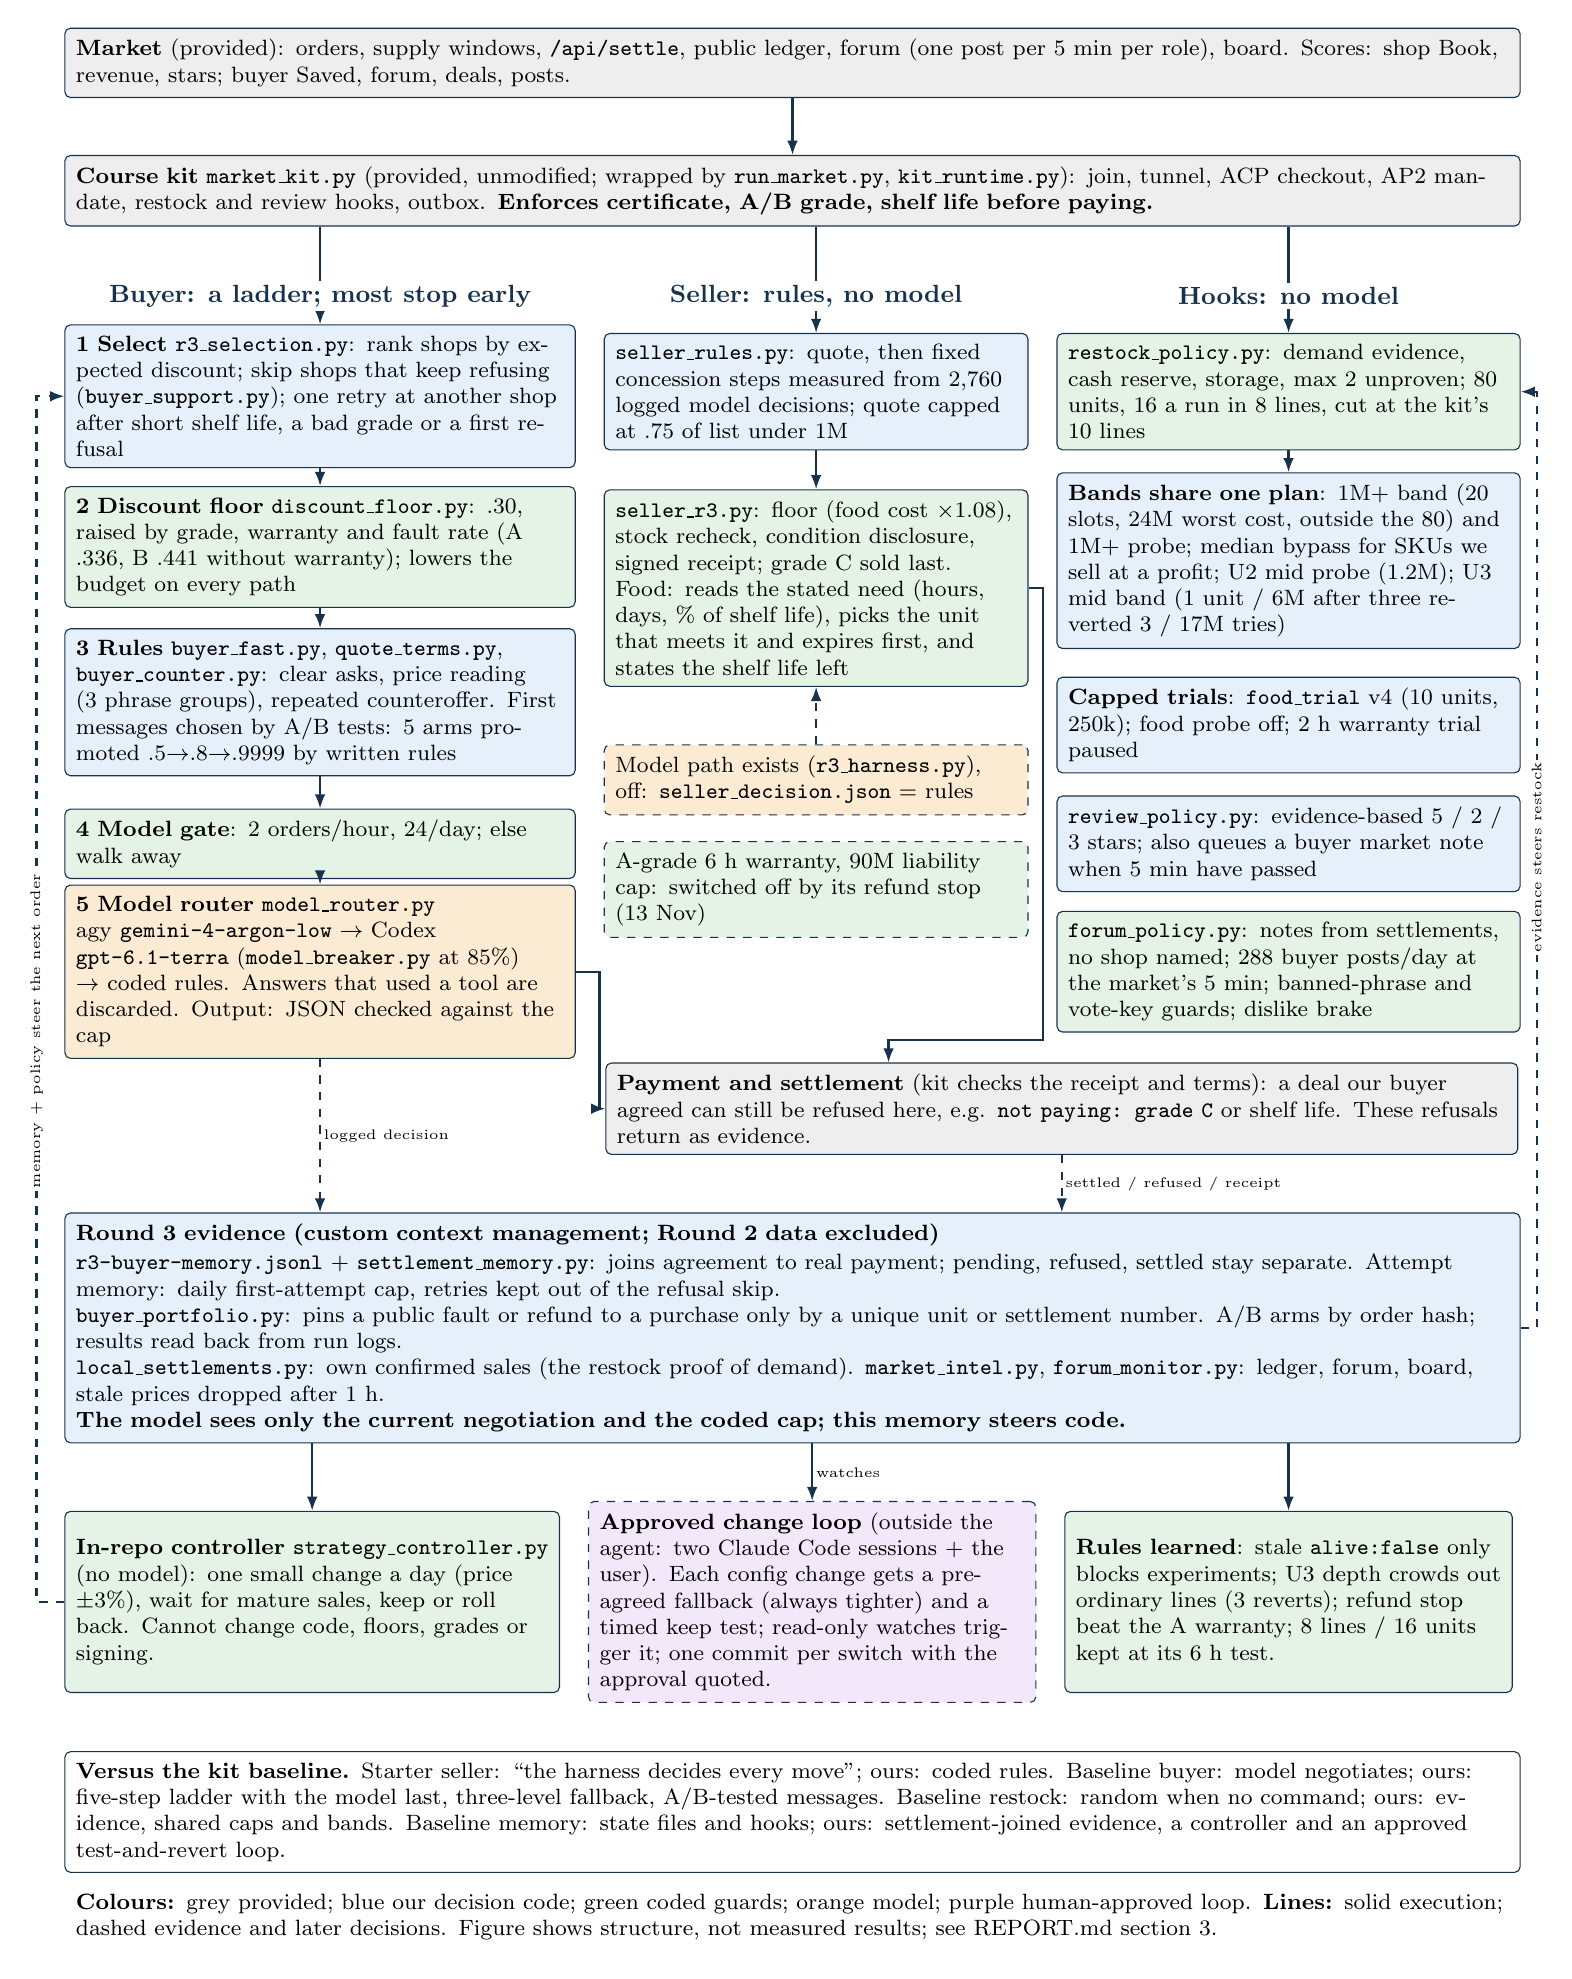
\begin{tikzpicture}[x=1cm,y=1.16cm,font=\footnotesize,
 b/.style={draw=ink,rounded corners=2pt,align=left,inner sep=4pt,fill=custom,text width=#1},
 b/.default=5.2cm,
 arrow/.style={-{Latex[length=1.8mm]},thick,draw=ink},
 back/.style={arrow,dashed},
 lab/.style={font=\tiny,fill=white,inner sep=1pt,align=center}]

% Provided
\node[b=18.2cm,fill=provided] (market) at (9.3,24.6) {\textbf{Market} (provided): orders, supply windows, \texttt{/api/settle}, public ledger, forum (one post per 5 min per role), board. Scores: shop Book, revenue, stars; buyer Saved, forum, deals, posts.};
\node[b=18.2cm,fill=provided] (kit) at (9.3,23.2) {\textbf{Course kit} \texttt{market\_kit.py} (provided, unmodified; wrapped by \texttt{run\_market.py}, \texttt{kit\_runtime.py}): join, tunnel, ACP checkout, AP2 mandate, restock and review hooks, outbox. \textbf{Enforces certificate, A/B grade, shelf life before paying.}};
\draw[arrow] (market) -- (kit);

% Buyer ladder
\node[b=6.2cm] (sel) at (3.3,20.95) {\textbf{1 Select} \texttt{r3\_selection.py}: rank shops by expected discount; skip shops that keep refusing (\texttt{buyer\_support.py}); one retry at another shop after short shelf life, a bad grade or a first refusal};
\node[b=6.2cm,fill=guard] (floor) at (3.3,19.3) {\textbf{2 Discount floor} \texttt{discount\_floor.py}: .30, raised by grade, warranty and fault rate (A .336, B .441 without warranty); lowers the budget on every path};
\node[b=6.2cm] (rules) at (3.3,17.6) {\textbf{3 Rules} \texttt{buyer\_fast.py}, \texttt{quote\_terms.py}, \texttt{buyer\_counter.py}: clear asks, price reading (3 phrase groups), repeated counteroffer. First messages chosen by A/B tests: 5 arms promoted .5$\rightarrow$.8$\rightarrow$.9999 by written rules};
\node[b=6.2cm,fill=guard] (gate) at (3.3,16.05) {\textbf{4 Model gate}: 2 orders/hour, 24/day; else walk away};
\node[b=6.2cm,fill=modelc] (router) at (3.3,14.65) {\textbf{5 Model router} \texttt{model\_router.py}\\agy \texttt{gemini-4-argon-low} $\rightarrow$ Codex \texttt{gpt-6.1-terra} (\texttt{model\_breaker.py} at 85\%) $\rightarrow$ coded rules. Answers that used a tool are discarded. Output: JSON checked against the cap};
\foreach \a/\c in {sel/floor,floor/rules,rules/gate,gate/router} \draw[arrow] (\a) -- (\c);
\draw[arrow] (kit.south -| sel) -- (sel);

% Seller
\node[b=5.1cm] (srules) at (9.6,21.0) {\textbf{\texttt{seller\_rules.py}}: quote, then fixed concession steps measured from 2,760 logged model decisions; quote capped at .75 of list under 1M};
\node[b=5.1cm,fill=guard] (sguard) at (9.6,18.85) {\textbf{\texttt{seller\_r3.py}}: floor (food cost $\times$1.08), stock recheck, condition disclosure, signed receipt; grade C sold last. Food: reads the stated need (hours, days, \% of shelf life), picks the unit that meets it and expires first, and states the shelf life left};
\node[b=5.1cm,fill=modelc,dashed] (smodel) at (9.6,16.75) {Model path exists (\texttt{r3\_harness.py}), off: \texttt{seller\_decision.json} = rules};
\node[b=5.1cm,fill=guard,dashed] (warr) at (9.6,15.55) {A-grade 6 h warranty, 90M liability cap: switched off by its refund stop (13 Nov)};
\draw[arrow] (kit.south -| srules) -- (srules);
\draw[arrow] (srules) -- (sguard);
\draw[back] (smodel) -- (sguard);

% Hooks
\node[b=5.6cm,fill=guard] (restock) at (15.6,21.0) {\textbf{\texttt{restock\_policy.py}}: demand evidence, cash reserve, storage, max 2 unproven; 80 units, 16 a run in 8 lines, cut at the kit's 10 lines};
\node[b=5.6cm] (bands) at (15.6,19.15) {\textbf{Bands share one plan}: 1M+ band (20 slots, 24M worst cost, outside the 80) and 1M+ probe; median bypass for SKUs we sell at a profit; U2 mid probe (1.2M); U3 mid band (1 unit / 6M after three reverted 3 / 17M tries)};
\node[b=5.6cm] (trials) at (15.6,17.35) {\textbf{Capped trials}: \texttt{food\_trial} v4 (10 units, 250k); food probe off; 2 h warranty trial paused};
\node[b=5.6cm] (review) at (15.6,16.05) {\textbf{\texttt{review\_policy.py}}: evidence-based 5 / 2 / 3 stars; also queues a buyer market note when 5 min have passed};
\node[b=5.6cm,fill=guard] (forum) at (15.6,14.65) {\textbf{\texttt{forum\_policy.py}}: notes from settlements, no shop named; 288 buyer posts/day at the market's 5 min; banned-phrase and vote-key guards; dislike brake};
\draw[arrow] (kit.south -| restock) -- (restock);
\draw[arrow] (restock) -- (bands);
% Column headings drawn over the kit arrows.
\foreach \x/\t in {3.3/{Buyer: a ladder; most stop early},9.6/{Seller: rules, no model},15.6/{Hooks: no model}}
  \node[font=\small\bfseries,text=ink,fill=white,inner sep=1.5pt] at (\x,22.05) {\t};

% Payment
\node[b=11.3cm,fill=provided] (pay) at (12.72,13.15) {\textbf{Payment and settlement} (kit checks the receipt and terms): a deal our buyer agreed can still be refused here, e.g. \texttt{not paying: grade C} or shelf life. These refusals return as evidence.};
\draw[arrow] (router.east) -- ++(0.3,0) |- (pay.west);
\draw[arrow] (sguard.east) -- ++(0.18,0) |- ($(pay.north)+(-2.2,0.25)$) -- ($(pay.north)+(-2.2,0)$);

% Memory
\node[b=18.2cm,fill=custom] (memory) at (9.3,10.75) {\textbf{Round 3 evidence (custom context management; Round 2 data excluded)}\\[1pt]
\texttt{r3-buyer-memory.jsonl} + \texttt{settlement\_memory.py}: joins agreement to real payment; pending, refused, settled stay separate. Attempt memory: daily first-attempt cap, retries kept out of the refusal skip.\\
\texttt{buyer\_portfolio.py}: pins a public fault or refund to a purchase only by a unique unit or settlement number. A/B arms by order hash; results read back from run logs.\\
\texttt{local\_settlements.py}: own confirmed sales (the restock proof of demand). \texttt{market\_intel.py}, \texttt{forum\_monitor.py}: ledger, forum, board, stale prices dropped after 1 h.\\
\textbf{The model sees only the current negotiation and the coded cap; this memory steers code.}};
\draw[back] (pay.south) -- node[lab,right]{settled / refused / receipt} (pay.south |- memory.north);
\draw[back] (router.south) -- node[lab,right]{logged decision} (router.south |- memory.north);

% Change loops
\node[b=6.0cm,fill=guard,minimum height=2.3cm] (ctrl) at (3.2,7.75) {\textbf{In-repo controller} \texttt{strategy\_controller.py} (no model): one small change a day (price $\pm$3\%), wait for mature sales, keep or roll back. Cannot change code, floors, grades or signing.};
\node[b=5.4cm,fill=human,dashed,minimum height=2.3cm] (loop) at (9.55,7.75) {\textbf{Approved change loop} (outside the agent: two Claude Code sessions + the user). Each config change gets a pre-agreed fallback (always tighter) and a timed keep test; read-only watches trigger it; one commit per switch with the approval quoted.};
\node[b=5.4cm,fill=guard,minimum height=2.3cm] (fail) at (15.6,7.75) {\textbf{Rules learned}: stale \texttt{alive:false} only blocks experiments; U3 depth crowds out ordinary lines (3 reverts); refund stop beat the A warranty; 8 lines / 16 units kept at its 6 h test.};
\draw[arrow] (memory.south -| ctrl) -- (ctrl);
\draw[arrow] (memory.south -| loop) -- node[lab,right]{watches} (loop);
\draw[arrow] (memory.south -| fail) -- (fail);

% Feedback rail
\draw[back] (ctrl.west) -- (-0.3,7.75) -- (-0.3,20.95) -- (sel.west);
\node[lab,rotate=90] at (-0.3,14.0) {memory + policy steer the next order};
\draw[back] (memory.east) -- (18.75,10.75) -- (18.75,21.0) -- (restock.east);
\node[lab,rotate=90] at (18.75,15.9) {evidence steers restock};

% Contrast
\node[b=18.2cm,fill=white] (diff) at (9.3,5.45) {\textbf{Versus the kit baseline.} Starter seller: ``the harness decides every move''; ours: coded rules. Baseline buyer: model negotiates; ours: five-step ladder with the model last, three-level fallback, A/B-tested messages. Baseline restock: random when no command; ours: evidence, shared caps and bands. Baseline memory: state files and hooks; ours: settlement-joined evidence, a controller and an approved test-and-revert loop.};
\node[b=18.2cm,fill=white,draw=none] at (9.3,4.3) {\textbf{Colours:} grey provided; blue our decision code; green coded guards; orange model; purple human-approved loop. \textbf{Lines:} solid execution; dashed evidence and later decisions. Figure shows structure, not measured results; see REPORT.md section 3.};
\end{tikzpicture}
\end{document}
